\PassOptionsToPackage{unicode}{hyperref}
\documentclass[aspectratio=1610, 9pt]{beamer}

% Load packages you need here
\usepackage{polyglossia}
\setmainlanguage{german}

\usepackage{csquotes}
\usepackage{graphicx}
\usepackage{siunitx}
\usepackage{amsmath}
\usepackage{amssymb}
\usepackage{mathtools}

\usepackage{hyperref}
\usepackage{bookmark}
\usepackage[backend=biber,autolang=hyphen,]{biblatex}
\addbibresource{references.bib}
\DefineBibliographyStrings{american}{andothers = {{et\,al\adddot}}}
% load the theme after all packages

\usetheme[
  showtotalframes, % show total number of frames in the footline
  % dark, % optional dark theme, uncomment to use
]{tudo}

% Put settings here, like
\unimathsetup{
  math-style=ISO,
  bold-style=ISO,
  nabla=upright,
  partial=upright,
  mathrm=sym,
}

\title{A deep learning based reconstruction of high-energy muons in IceCube}
\author{Leander Flottau}
%\institute{Astroteilchenphysik \\  Fakultät: Physik}
\titlegraphic{\includegraphics[width=0.7\textwidth]{images/tudo-title-2.jpg}}
\begin{document}
\maketitle
\begin{frame}
  \frametitle{Table of Contents}
  \tableofcontents
\end{frame}  
\section{Introduction}
\begin{frame}
  \frametitle{Introduction: prompt muons}
  \begin{itemize}
    \item Atmospheric muons divided into a prompt and a conventional component
    \item Conventional component: 
    \begin{align}
      \pi^{\pm} \rightarrow \mu^{\pm}+\nu_{\mu}(\bar{\nu}_{\mu}), \\
      K^{\pm} \rightarrow \mu^{\pm}+\nu_{\mu}(\bar{\nu}_{\mu})
    \end{align}
    \item Lifetime: $\tau_{\pi}\approx 2.6*10^{-8} \si{\second}$, $\tau_{K}\approx 1.2*10^{-8} \si{\second}$
    \item Prompt component: originate from particles with a significantly shorter lifetime like the D-meson ($\tau_{D}\approx 10^{-12}\si{\second}$) and unflavored mesons
    \item Short lifetime \rightarrow decay before interaction
    \item Main differences to conventional muons
    %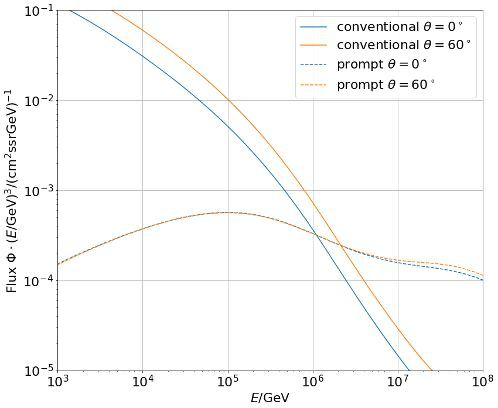
\includegraphics[scale=0.2]{prompt conventional flux ludwig}
    \begin{itemize}
      \item Isotropic angular distribution
      \item Energy spectrum: prompt component becomes dominant for high energies
    \end{itemize}
  \end{itemize}
\end{frame}
\begin{frame}
  \frametitle{Introduction: Prompt muons}
  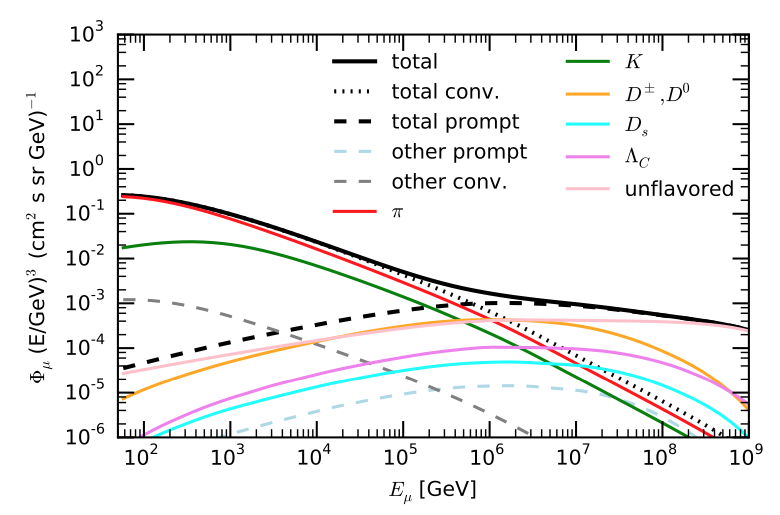
\includegraphics[scale=0.25]{Plots/Prompt vs conventional flux}
  \begin{itemize}
    \item Main differences to conventional muons \cite{fedynitch2015calculation}
    %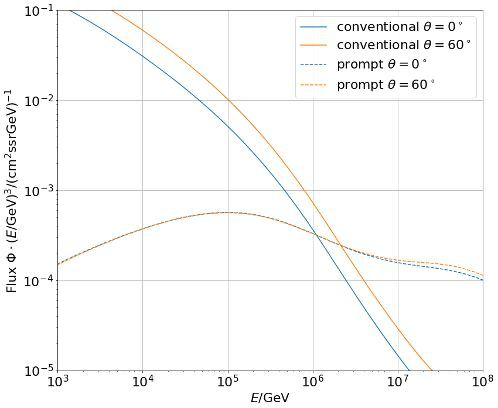
\includegraphics[scale=0.2]{prompt conventional flux ludwig}
    \begin{itemize}
      \item Isotropic angular distribution
      \item Energy spectrum: prompt component becomes dominant for high energies
    \end{itemize}
%    \item conventional dominant for energies up to $E_{\mu}\approx\SI{5e5}{\giga\electronvolt}$
  \end{itemize}
\end{frame}
\begin{frame}
  \frametitle{Introduction: IceCube Neutrino Observatory}
  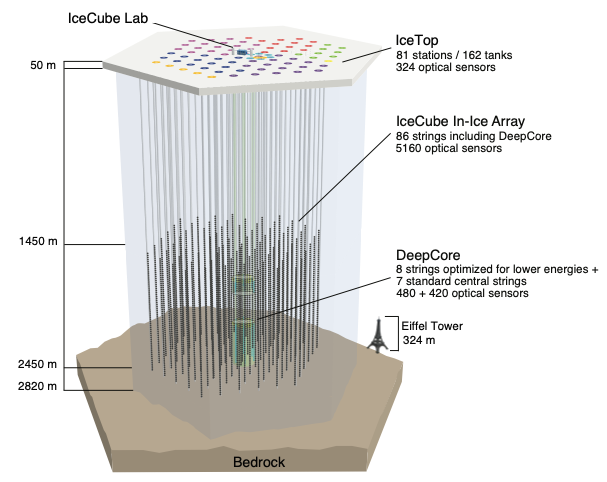
\includegraphics[scale=0.3]{Plots/IceCube schematic}
  \begin{itemize}
    \item Kilometer-scale cherenkov detector \cite{Aartsen_2017}
    \item Designed to detect neutrinos, atmospheric muons are background
    \item $\SI{3000}{\hertz}$ event rate \rightarrow fast runtime needed
  \end{itemize}
\end{frame}
\begin{frame}
  \frametitle{Introduction}
  \begin{itemize}
    \item Detecting the prompt component of the atmospheric muon flux requires efficient energy reconstruction
    \item Focus on the leading muon: most energetic muon in a bundle
    \item Two important values to reconstruct:
    \begin{itemize}
      \item Bundle energy at detector entry
      \item Energy of the leading muon at detector entry
    \end{itemize}
    \item Neural networks: Good results in similar tasks
  \end{itemize}
\end{frame}
\begin{frame}
  \frametitle{Introduction: Input features}
  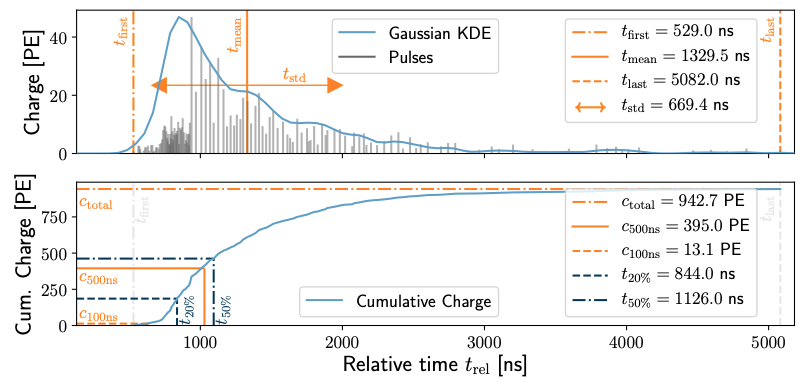
\includegraphics[scale=0.35]{Plots/Data input}
  \begin{itemize}
    \item DNN input features: pulse series summarized by nine features \cite{Abbasi_2021}
    \item Only three used to minimize runtime
    \begin{itemize}
      \item $c_{total}$
      \item $t_{first}$
      \item $t_{std}$
    \end{itemize}
  \end{itemize}
\end{frame}
\section{Motivation}
\begin{frame}
  \frametitle{Motivation}
  \begin{itemize}
    \item Muon puzzle: Unexplained difference between measurement and simulation of muon number
    \item Likely reason: Hadronic interactions
    \item Improving knowledge of hadronic interactions
  \end{itemize}
\end{frame}
\section{Reconstruction performance}
\subsection{Bundle energy}
\begin{frame}
  \frametitle{Bundle energy}
  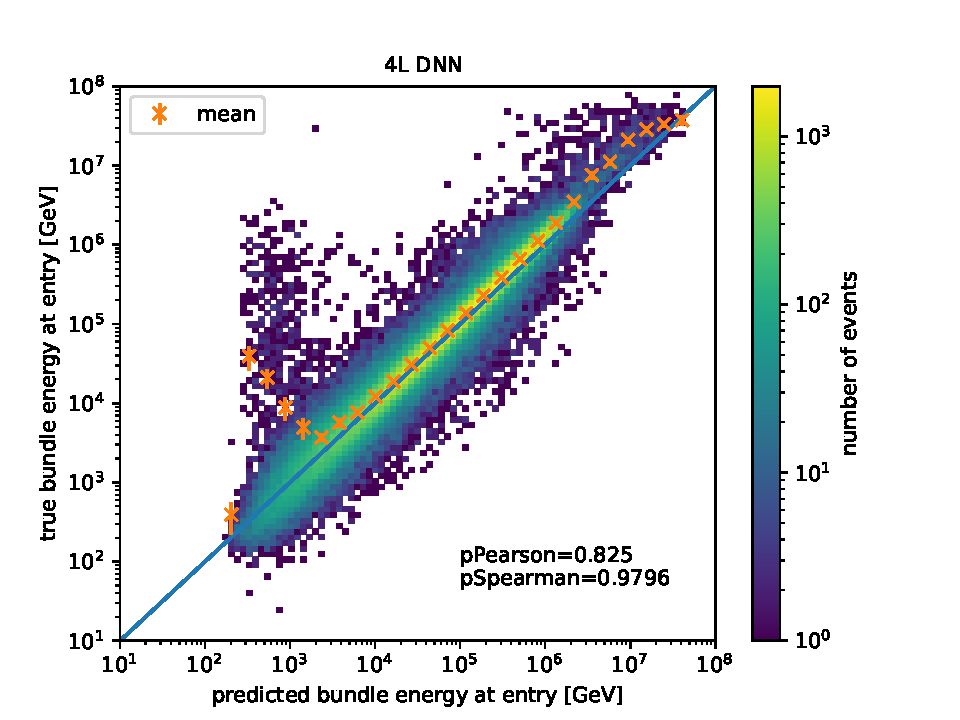
\includegraphics[scale=0.45]{Plots/correlation_4L_bundle.pdf}
  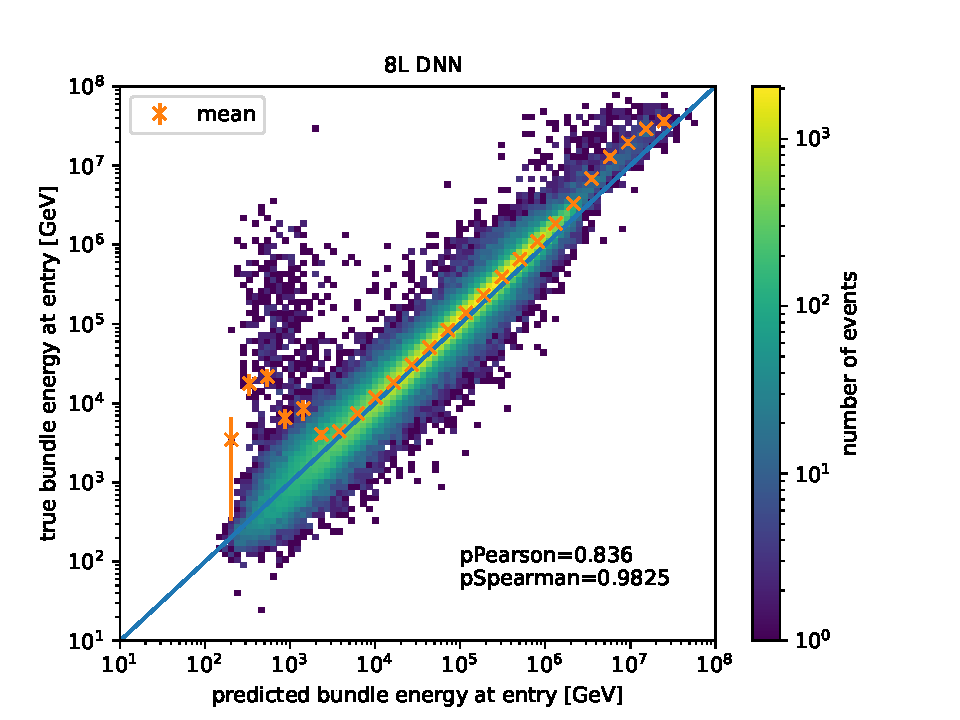
\includegraphics[scale=0.45]{Plots/correlation_8L_bundle.pdf}
  \begin{itemize}
    \item Some significant smearing for lower energies
    \item Bigger network doesn't seem to be visibly better, except for slight improvements in correlation
    \item Bias towards underestimation for higher energies
  \end{itemize}
\end{frame}
\begin{frame}
  \frametitle{Bundle energy quality cut}
  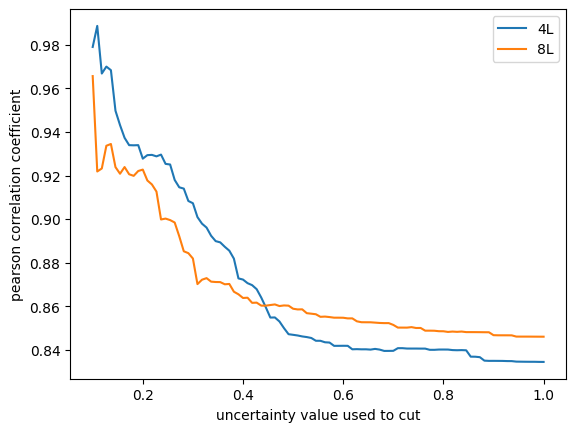
\includegraphics[scale=0.4]{Plots/Pearson depending on cut}
  \begin{itemize}
    \item Uncertainty estimated by separate subnetwork
    \item Improve reconstruction by cutting for low uncertainty
    \item Value to cut depends on application: How much data loss is affordable?
    \item Correlation coefficient can be used as an indication
  \end{itemize}
\end{frame}
\begin{frame}
  \frametitle{Bundle energy quality cut}
  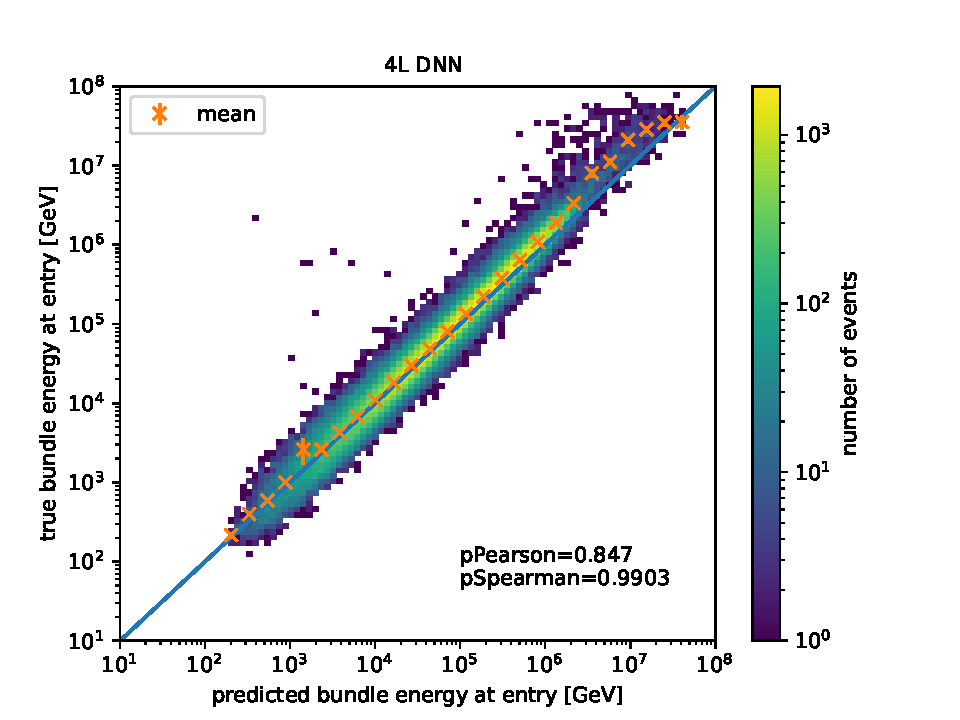
\includegraphics[scale=0.4]{Plots/correlation_4L_bundle_cut.pdf}
  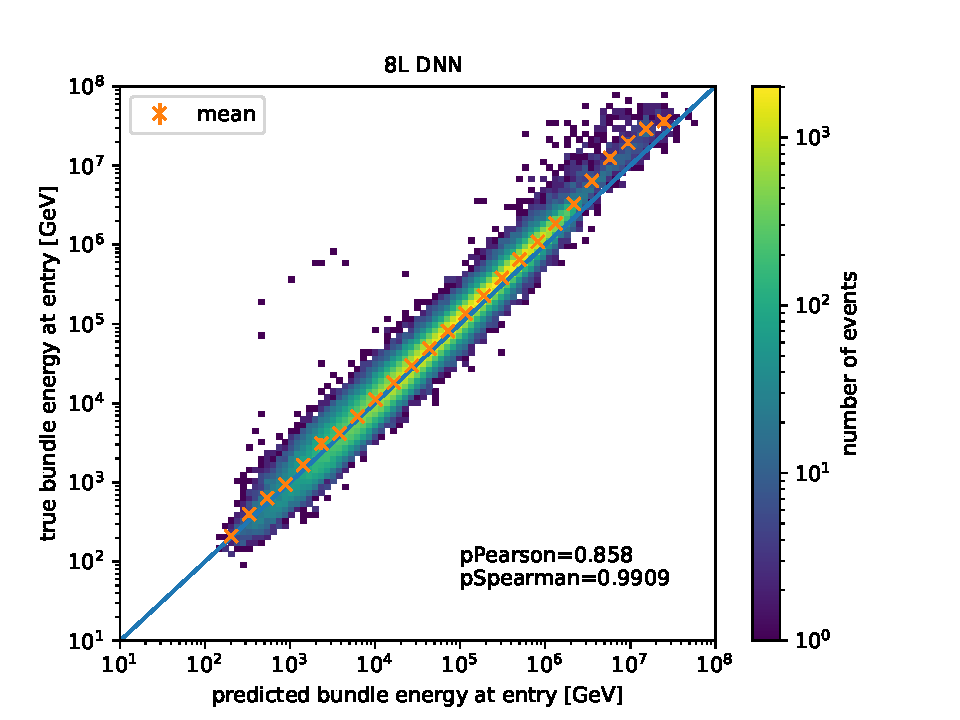
\includegraphics[scale=0.4]{Plots/correlation_8L_bundle_cut.pdf}
  \begin{itemize}
    \item Fixed uncertainty cut for both networks $\sigma=\num{0.5}$
    \item Events remainig: $\SI{84,9}{\percent}$ (4L) and  $\SI{87,1}{\percent}$
    \item Smearing on low energies almost completely eliminated, bias still present
    \item Better linear correlation
    \item Limited amount of statistic \rightarrow Bigger cuts hard to evaluate
  \end{itemize}
\end{frame}
\begin{frame}
  \frametitle{Comparison to non DNN based reconstruction}
  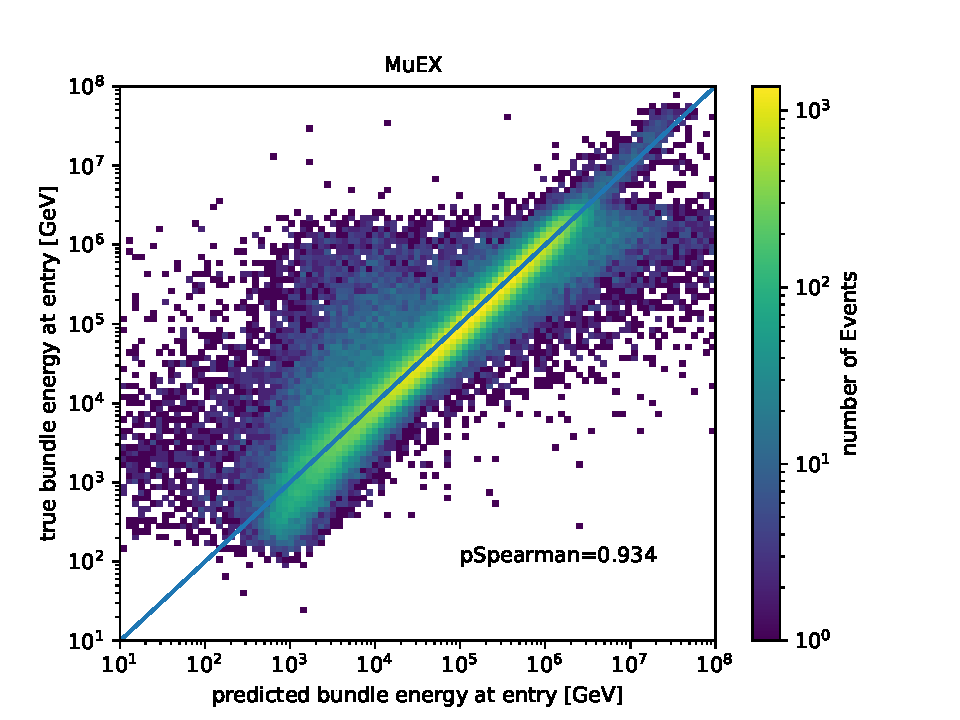
\includegraphics[scale=0.45]{Plots/correlation_muex_bundle.pdf}
  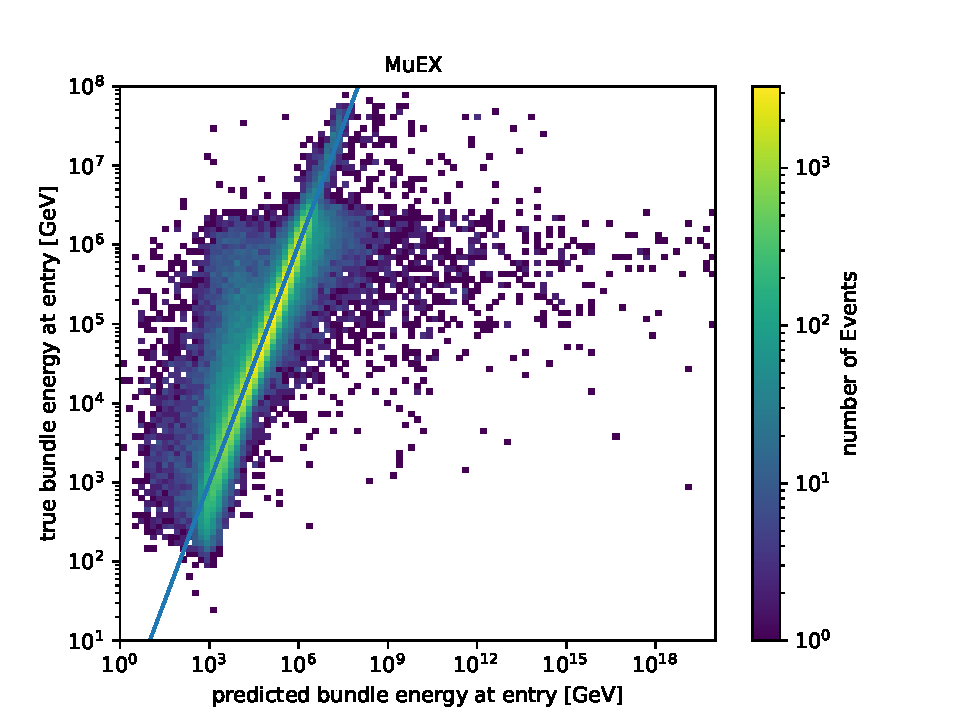
\includegraphics[scale=0.45]{Plots/correlation_muex_bundle2.pdf}
  \begin{itemize}
    \item Considerably stronger overall smearing than for the DNN
    \item Extreme overestimation for high energies (up to $\SI{e27}{\giga\electronvolt}$)
    \item Non DNN based approach shows significantly worse reconstruction especially in the important high energy region
  \end{itemize}
\end{frame}
\begin{frame}
  \frametitle{Resulting energy spectrum for high bundle energies: DNN}
  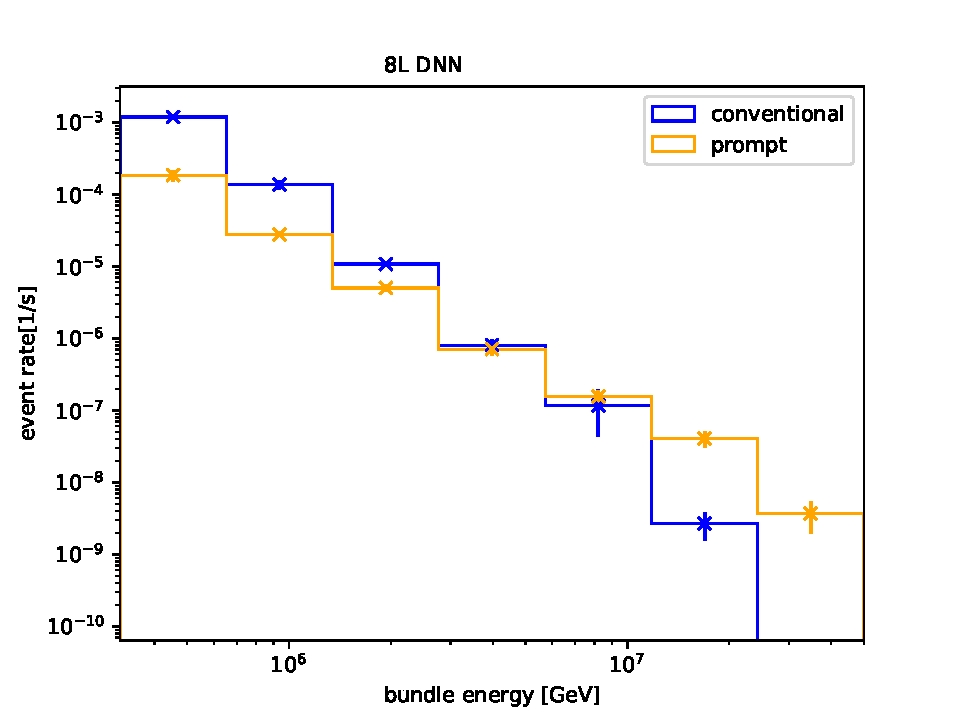
\includegraphics[scale=0.3]{Plots/spectrum_8L_bundle.pdf}
  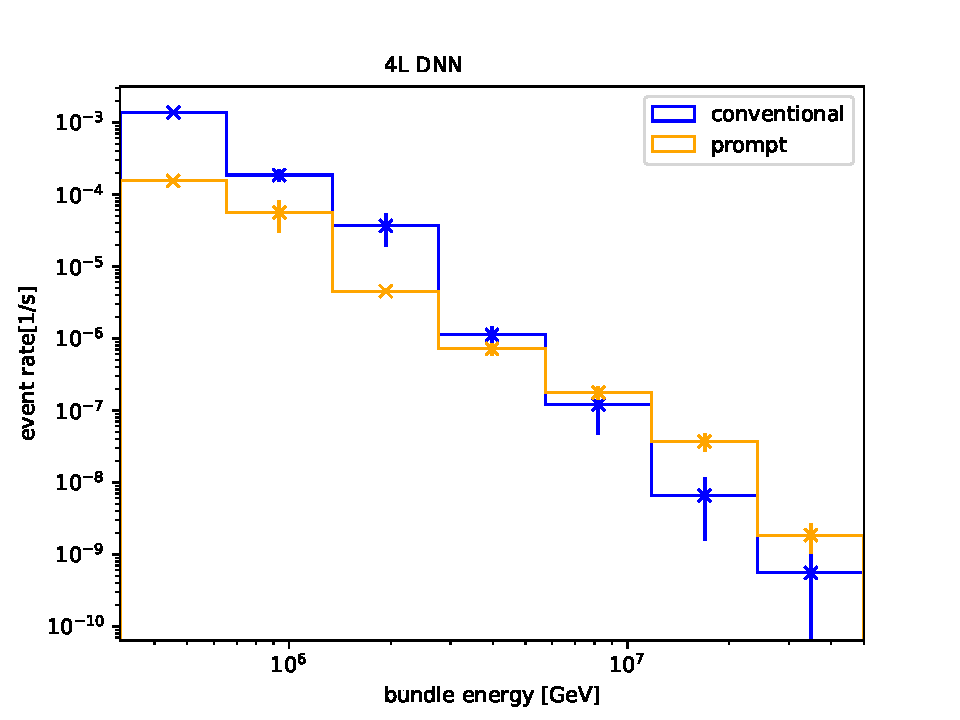
\includegraphics[scale=0.3]{Plots/spectrum_4L_bundle.pdf}
  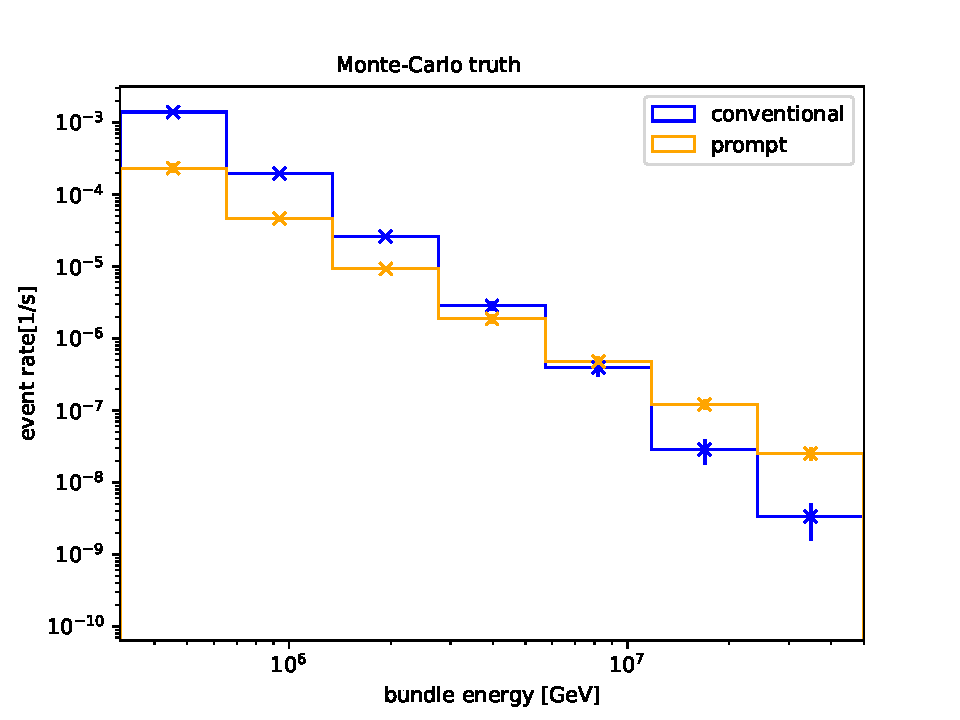
\includegraphics[scale=0.3]{Plots/spectrum_MC_bundle.pdf}
  \begin{itemize}
    \item All plots weighted using GaisserH3a
    \item Both DNNs generally show a good reconstruction of the high energy spectrum. the systematic underestimation leads to a slightly lower event rate in the highest energy bins
  \end{itemize}
\end{frame}
\begin{frame}
  \frametitle{Resulting energy spectrum for high bundle energies: MuEX}
  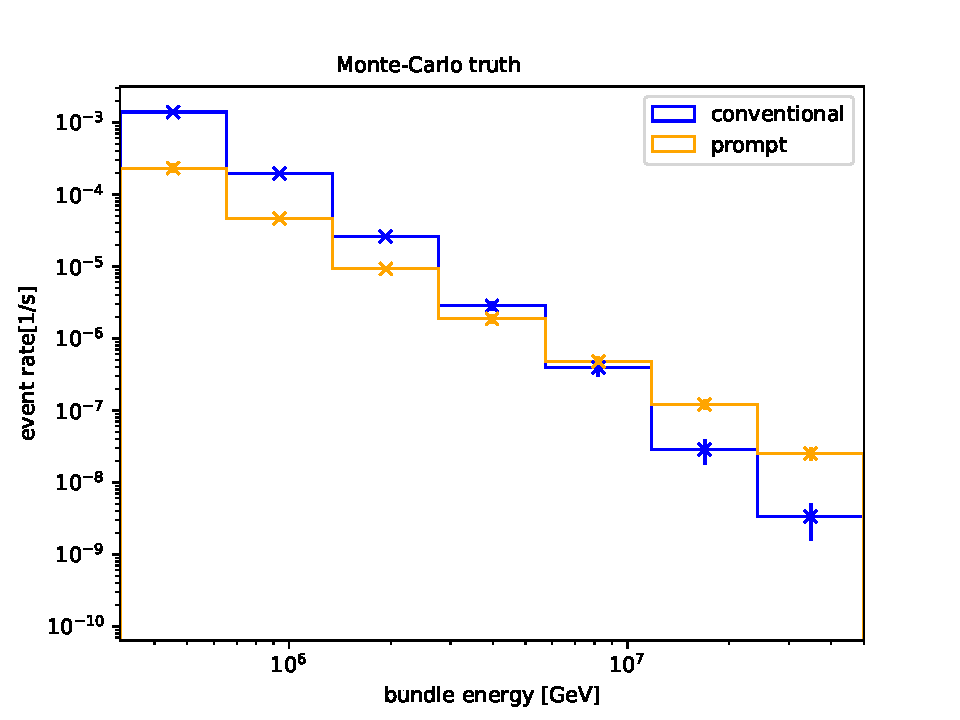
\includegraphics[scale=0.45]{Plots/spectrum_MC_bundle.pdf}
  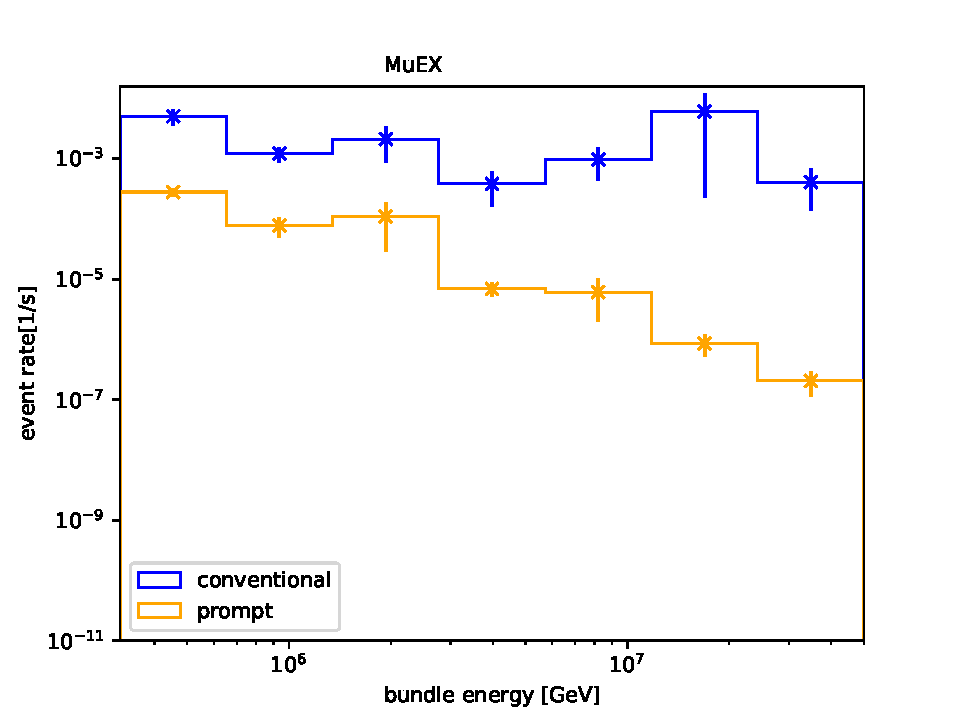
\includegraphics[scale=0.45]{Plots/spectrum_muex_bundle.pdf}
  \begin{itemize}
    \item Unrealistically high event rate for very high energies
    \item The MuEX Fit does not even see the prompt component as dominant for high energies. \rightarrow strong overestimation makes it unusable for the purpose of this analysis
  \end{itemize}
\end{frame}
\subsection{Energy of the leading muon}
\begin{frame}
  \frametitle{Energy of the leading muon}
  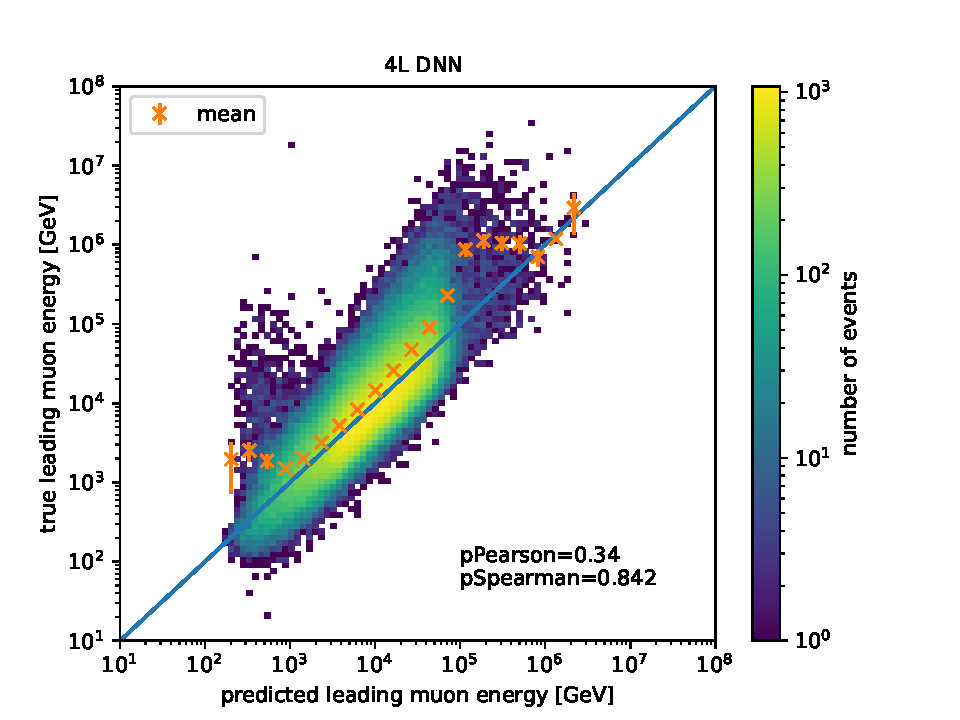
\includegraphics[scale=0.45]{Plots/correlation_4L_entry.pdf}
  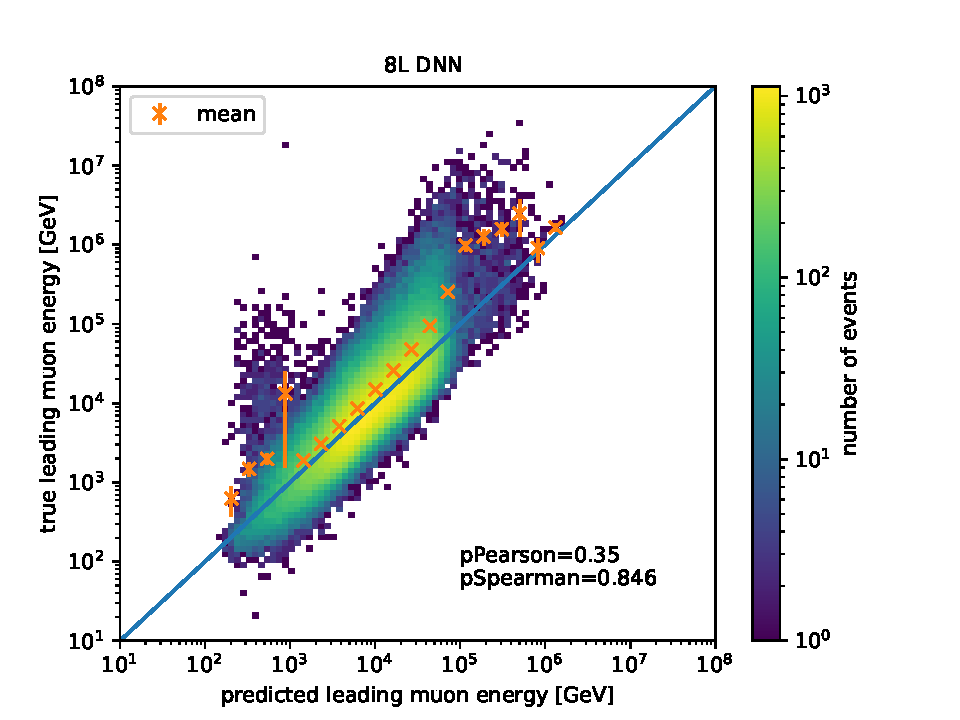
\includegraphics[scale=0.45]{Plots/correlation_8L_entry.pdf}
  \begin{itemize}
    \item As expected: Results much worse compared to bundle energy (especially linear correlation)
    \item Generally higher spread 
    \item Strong underestimation in high energy region
    \item Reconstructed energy rarely above $\SI{100}{\tera\electronvolt}$ (only $\SI{8,9}{\percent}$ of events above $\SI{100}{\tera\electronvolt}$ were predicted above $\SI{100}{\tera\electronvolt}$)
  \end{itemize}
\end{frame}
\begin{frame}
  \frametitle{Leading muon energy spectrum}
  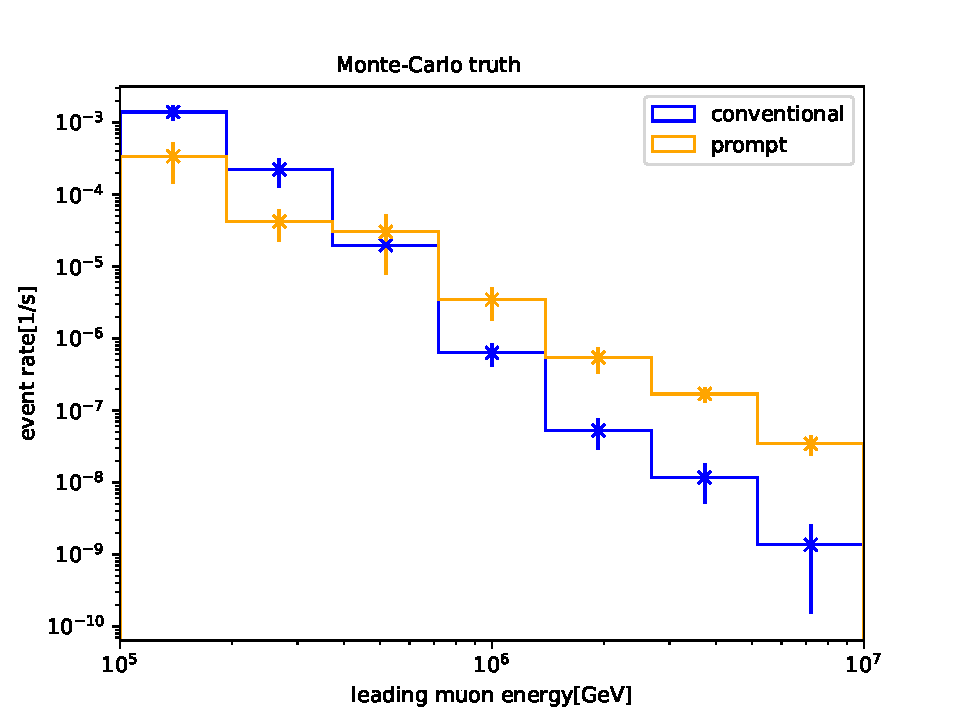
\includegraphics[scale=0.3]{Plots/spectrum_MC_entry.pdf}
  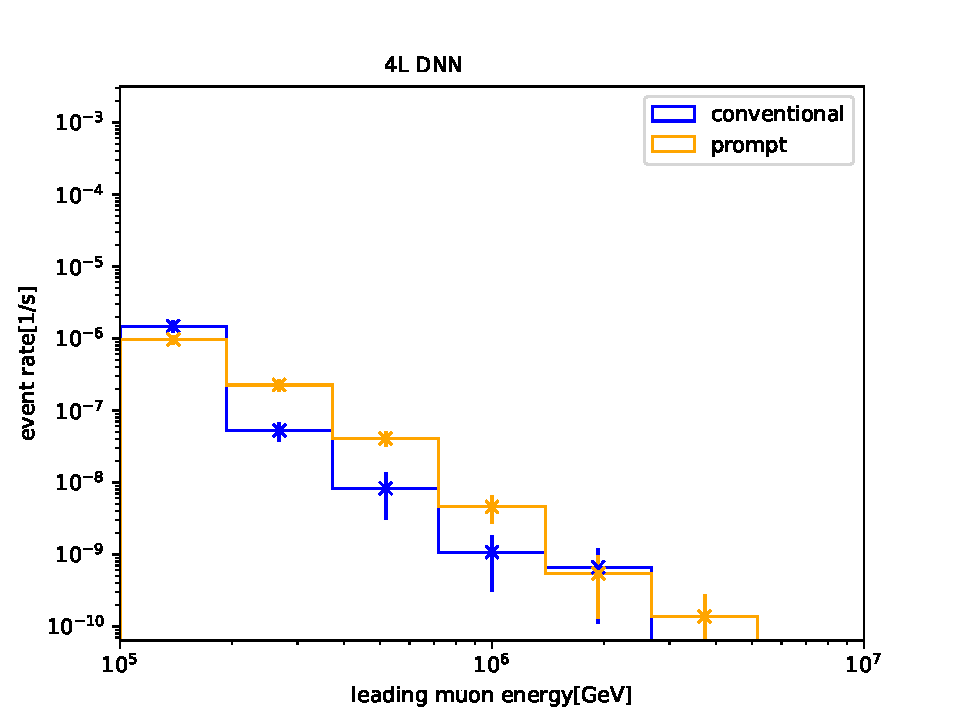
\includegraphics[scale=0.3]{Plots/spectrum_4L_entry.pdf}
  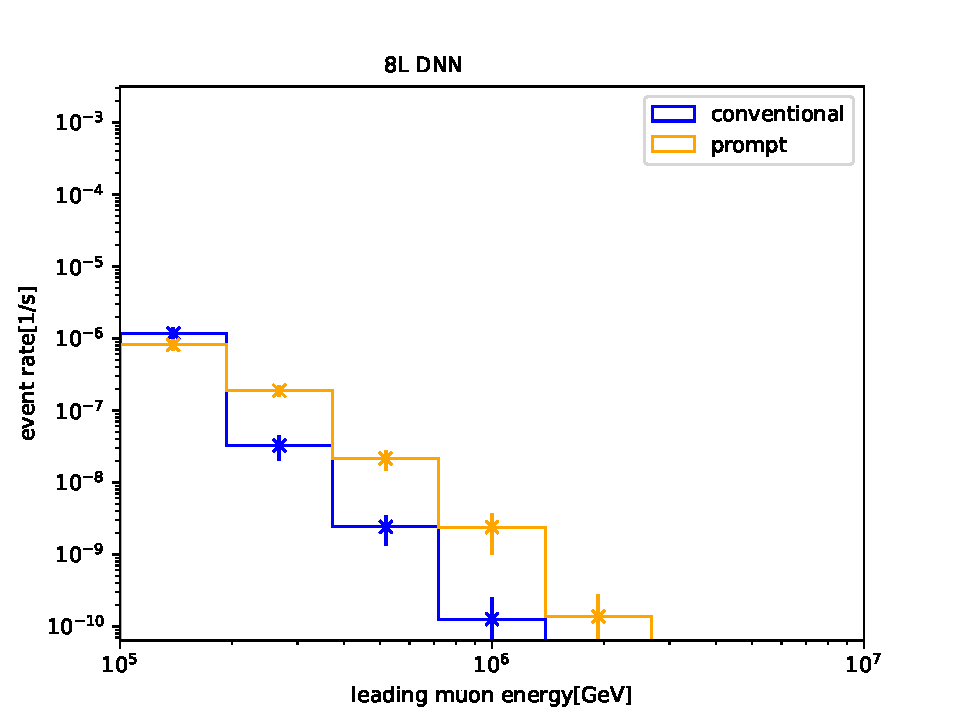
\includegraphics[scale=0.3]{Plots/spectrum_8L_entry.pdf}
  \begin{itemize}
    \item Prompt sensitivity is better in this label, as seen in Monte-Carlo
    \item Event rate at least three orders of magnitude too low for both DNNs
    \item Spectrum much steeper than it should be
    \item Strong underestimation in the highest energy bins as seen in correlation plots previously
  \end{itemize}
\end{frame}
%\begin{frame}
  %\frametitle{Energy of the leading muon quality cut}
  %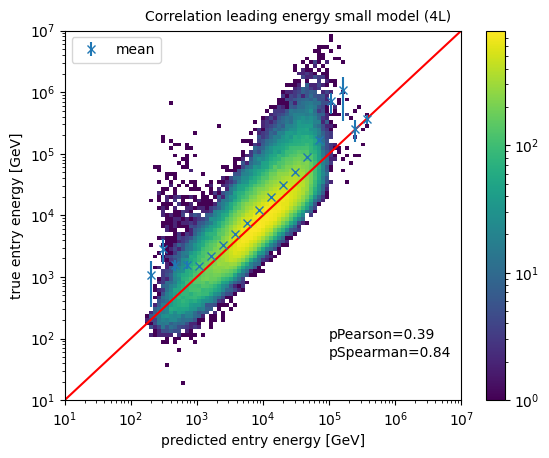
\includegraphics[scale=0.3]{correlation leading energy small dnn cut}
  %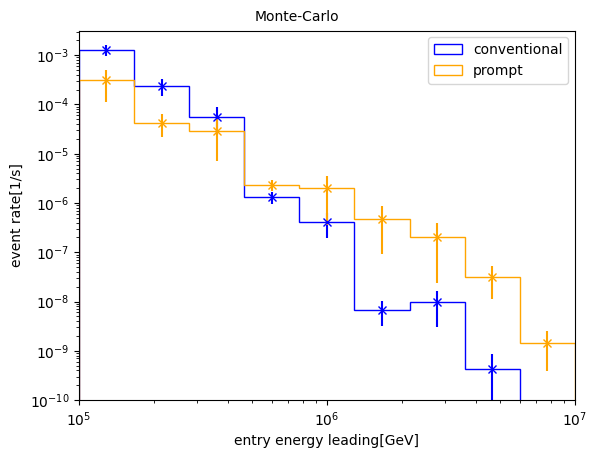
\includegraphics[scale=0.3]{muon flux monte carlo entry cut}
  %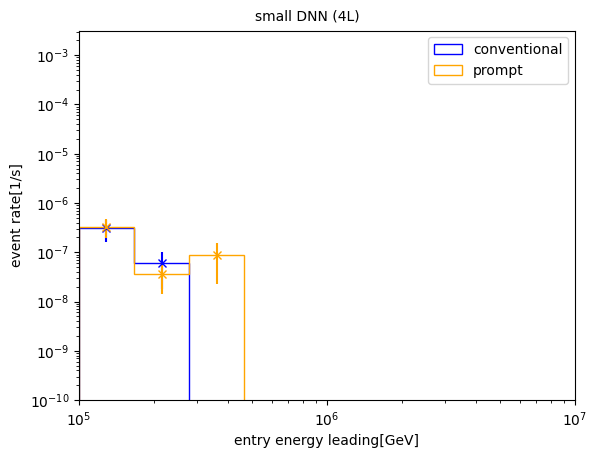
\includegraphics[scale=0.3]{muon flux small dnn entry cut}
  %\begin{itemize}
    %\item Even very small quality cuts eleminate disproportionately high amounts of prompt events in the important energy region
    %\item Qualitiy cut for $93.8\%$ leaves only $2s3\%$ of events predicted over $100 \si{\tera\electronvolt}$
  %\end{itemize}
%\end{frame}
\begin{frame}
  \frametitle{Leading muon energy reconstruction: leading fraction}
  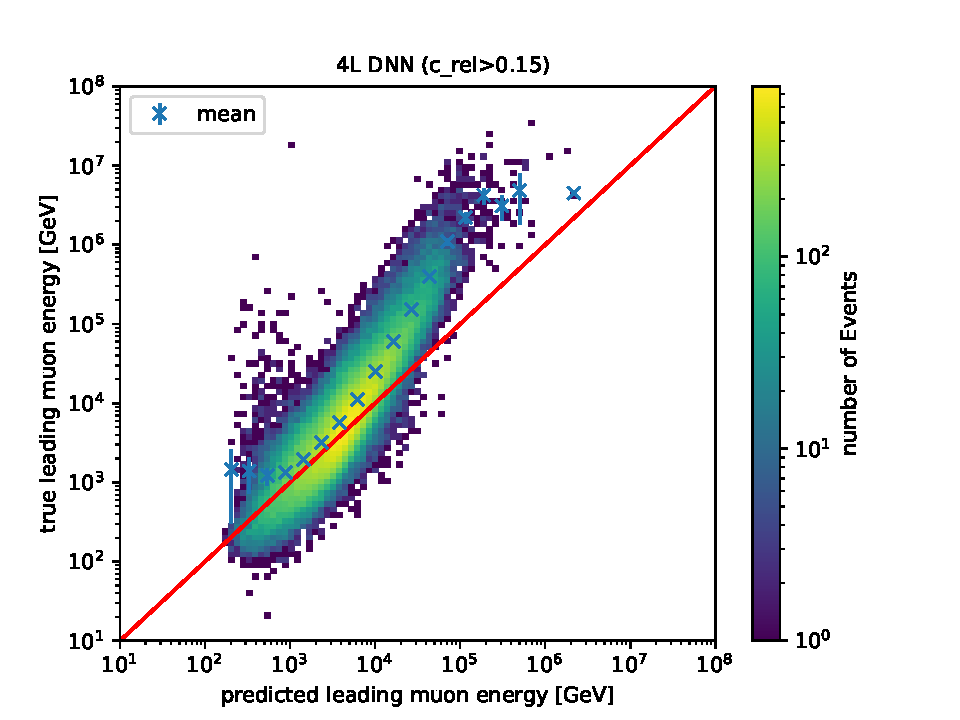
\includegraphics[scale=0.45]{Plots/spectrum_4L_entry_rel_cut}
  \begin{itemize}
    \item Assumption: if the network is actually able to predict, how dominant the leading muon is within the bundle, this should be easier to reconstruct for higher leading fractions
    \item Cut for events with more dominant leading muons $E_{lead}/E_{bundle}>\num{0.15}$
    \item Resulting energy reconstruction is significantly worse for higher energies
  \end{itemize}
\end{frame}
\begin{frame}
  \frametitle{Correlation of bundle energy and leading fraction}
  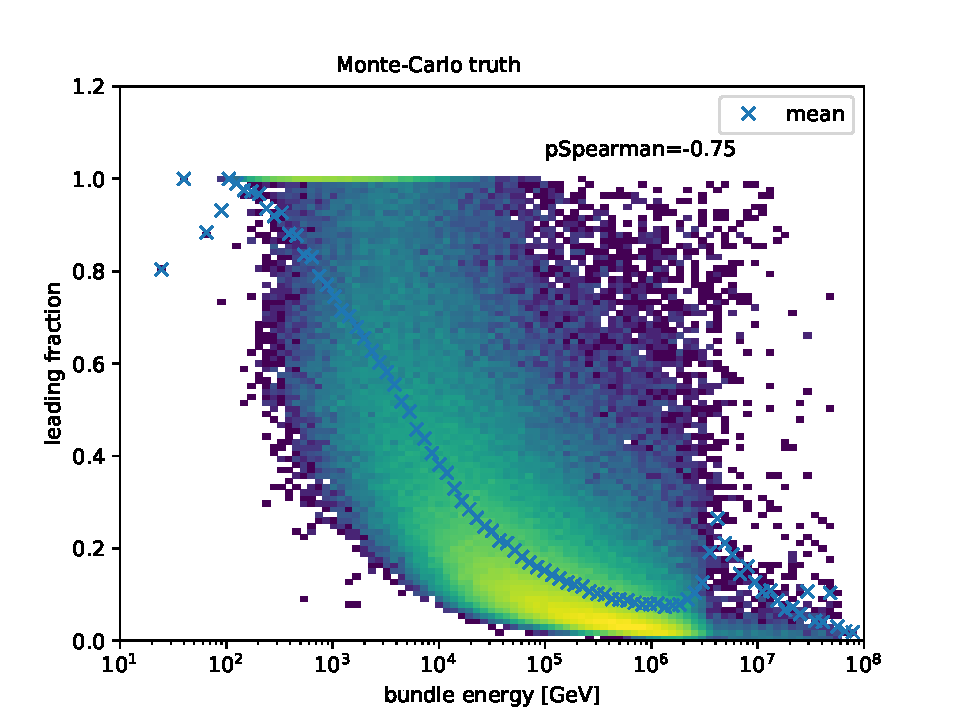
\includegraphics[scale=0.45]{Plots/correlation_MC_bundle_leading.pdf}
  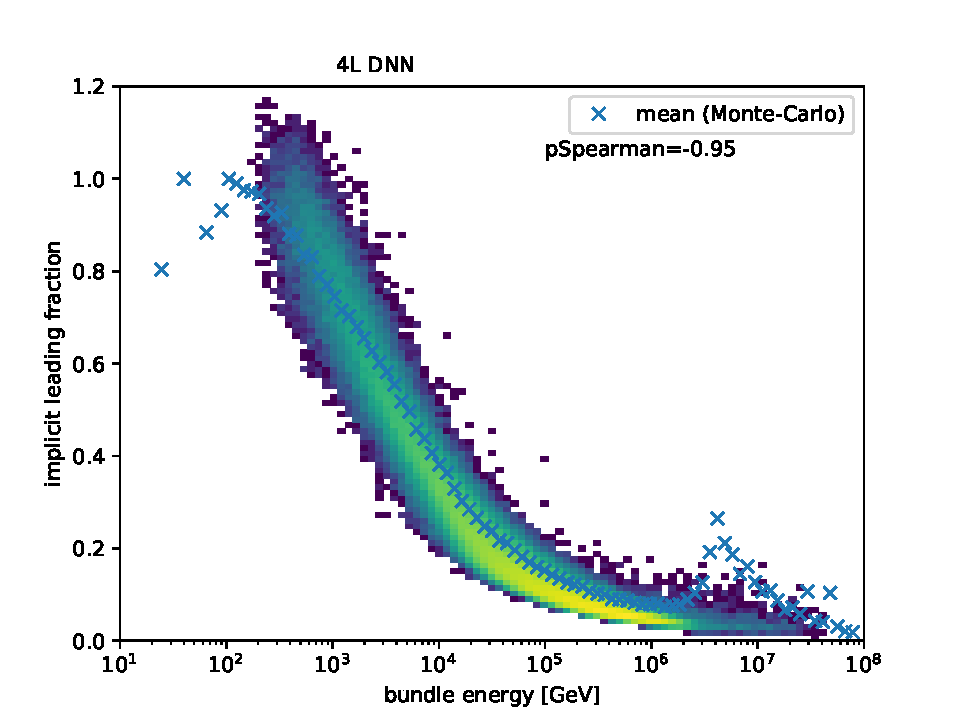
\includegraphics[scale=0.45]{Plots/correlation_4L_bundle_leading_implicit.pdf}
  %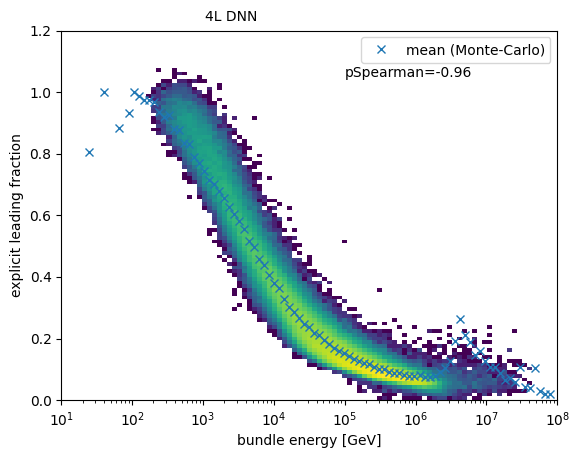
\includegraphics[scale=0.3]{energy leading fraction correaltion small dnn explicit}
  \begin{itemize}
    \item Reconstructed leading fraction shows very strong correlation to bundle energy
    \item Spearman correlation coefficient: $\rho_{MC}=\num{-0.75}$, $\rho_{DNN}=\num{-0.95}$
    \item Prediction as energy based mean instead of actual prediction of the leading fraction
    \item Automatically assuming a low leading fraction for high energies explains the underestimation
%    \item Correlation for explicit leading fraction lower \rightarrow possibly better to train problems separately 
  \end{itemize}
\end{frame}
\subsection{Optimization}
\begin{frame}
  \frametitle{Optimization: Leading muon energy}
  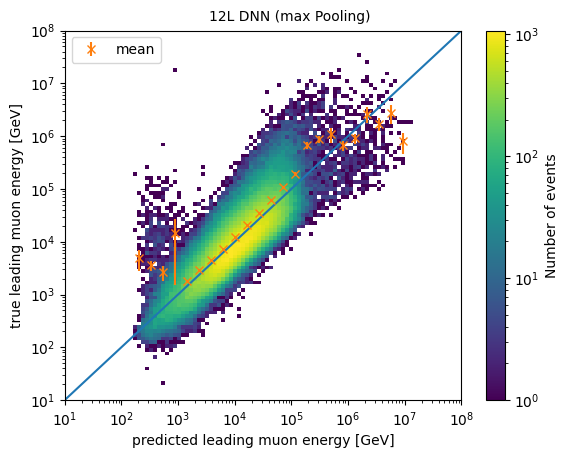
\includegraphics[scale=0.45]{Plots/Correlation leading 12L max}
  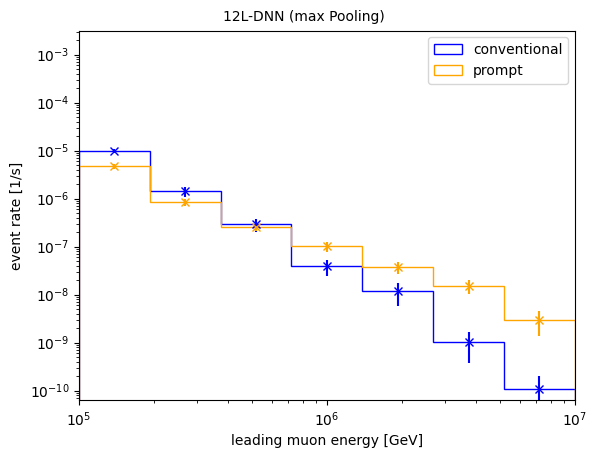
\includegraphics[scale=0.45]{Plots/muon flux calculated 12L max}
  \begin{itemize}
    \item To improve the leading moun reconstruction, further changes can be made
    \item Increasing number of convolutional layers and number of filters, max instead of average pooling
    \item Use independently calculated leading fraction
    \item Better coverage of the high energy region: $\SI{22,3}{\percent}$ compared to $\SI{8,9}{\percent}$
    \item Leads to better spectrum and prompt sensitivity
  \end{itemize}
\end{frame}
\begin{frame}
  \frametitle{Optimization: Leading muon energy}
  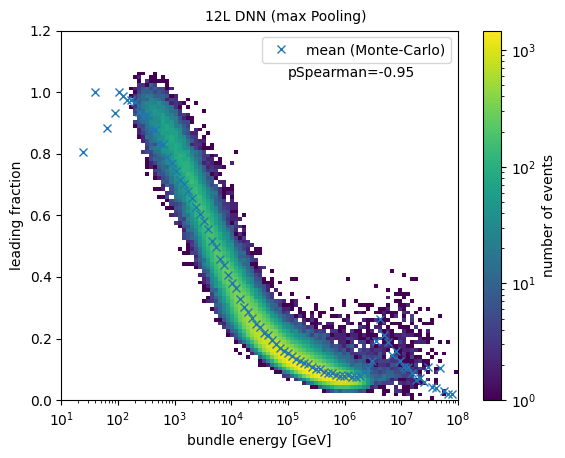
\includegraphics[scale=0.4]{Plots/Correlation bundle leading 12L}
  \begin{itemize}
    \item Underlying problem remains the same
    \item Event rate still underestimated \rightarrow bundle energy better alternative
    \item Potential limited unless leading fraction is separated from bundle energy
    \item Not easily achieved by increasing network size
  \end{itemize}
\end{frame}
%\begin{frame}
%  \frametitle{Optimization: Bundle energy}
%  \includegraphics[scale=0.5]{}
%  \includegraphics[scale=0.5]{}
% \begin{itemize}
%    \item Bundle energy reconstruction already works well, even for small networks
%    \item Try to improve the small network
%    \item Changing from average to max pooling \rightarrow easy way to improve linear correlation and prompt sensitivity
%    \item Does not increase the runtime
%  \end{itemize}
%\end{frame}
\section{Runtime comparison}
\begin{frame}
  \frametitle{Runtime comparison}
  \begin{columns}
    \column{0.5\textwidth}
      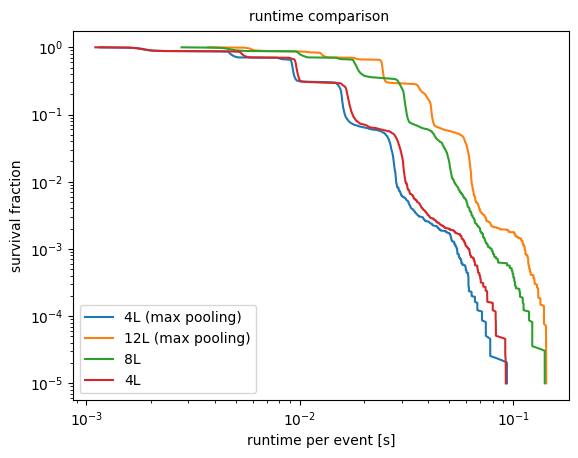
\includegraphics[scale=0.45]{Plots/Runtime comparison}
    \column{0.5\textwidth}  
      \begin{itemize}
        \item Median:
        \begin{itemize}
          \item $\mathrm{median}(t_{4L})=\SI{0,0096}{\second}$
          \item $\mathrm{median}(t_{8L})=\SI{0,0185}{\second}$ 
          \item $\mathrm{median}(t_{12L})=\SI{0,0247}{\second}$
        \end{itemize}
        \item Median($t_{8L}/t_{4L}=\num{1,88}$) \rightarrow small DNN almost twice as fast
        \item Faster in $99,9\%$ of cases
      \end{itemize}
  \end{columns}
\end{frame}
\section{Summary}
\begin{frame}
  \frametitle{Summary}
  \begin{itemize}
    \item Good reconstruction for the bundle energy
    \item DNNs outperform non DNN based alternative
    \item Leading muon energy is not correctly learned
    \item Bigger DNN provides no significant performance improvement in relation to runtime increase
  \end{itemize}
\end{frame}
\section{Outlook}
\begin{frame}
  \frametitle{Outlook}
  \begin{itemize}
    \item Improve leading muon energy prediction
    \item Can this be properly trained or are the underlying physics just not there?
    \item Evaluate event multiplicity reconstruction
    \item Simulate and try to train on stochasticity
    \item Single label reconstruction
  \end{itemize}
\end{frame}
\begin{frame}
  \frametitle{Bibliography}
  \printbibliography	
\end{frame}
\end{document}